
%使用XeLaTeX编译
%版权所有,翻版必究
%本文件由程序自动生成,任何修改将被覆盖
%2019 年 01 月 23 日




\FloatBarrier
\section{
RadialGradient
}\label{c000015s000012}


%begin图片
\begin{figure}[htb] %浮动体 here and top ...
%there must use marginnote not use marginnote ...
\marginnote{\setlength\fboxsep{2pt}\fbox{\footnotesize{\kaishu\figurename\,}\footnotesize{\ref{p000028}}}}\centering %中心对齐
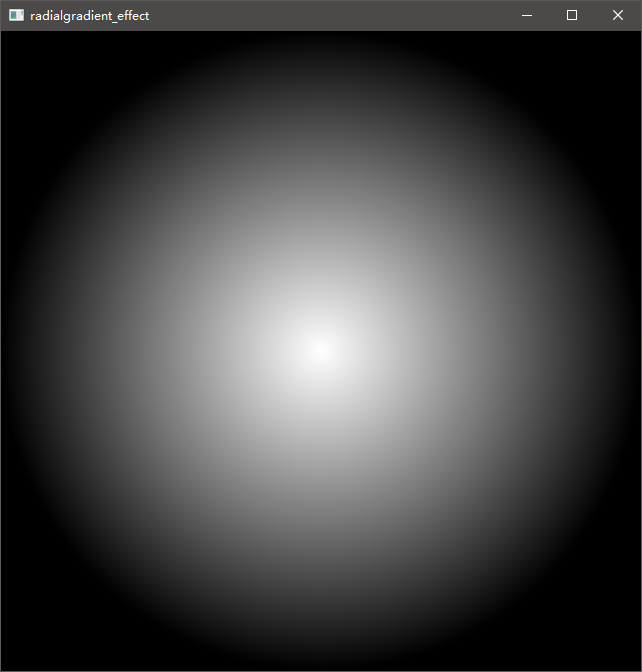
\includegraphics[width=0.95\textwidth]{../chapter06/radialgradient_effect/the_app.png} %图片路径
\caption{RadialGradient} %标题
\label{p000028} %索引
\end{figure}
%end图片


%\begin{spacing}{1.0}
\refstepcounter{filesourcenumber}\label{f000062}    %增加源代码编号
\FloatBarrier                                  %强制完成浮动体布局
\begin{thebookfilesourceone}[escapeinside={(*@}{@*)},
caption=GoodLuck,
title=\filesourcenumbernameone \thefilesourcenumber
]
/*radialgradient_effect/main.qml*/
import QtQuick 2.9
import QtGraphicalEffects 1.12

Rectangle {
    id : idRoot
    width: 640;
    height: 640;
    color: Qt.rgba(0.8,0.8,0.8,1);

    RadialGradient {
        anchors.fill: parent
        gradient: Gradient {
            GradientStop { position: 0.0; color: "white" }
            GradientStop { position: 0.5; color: "black" }
        }
    }

}(*@\marginpar[\hfill\setlength\fboxsep{2pt}\fbox{\footnotesize{\kaishu\parbox{1em}{\setlength{\baselineskip}{2pt}\filesourcenumbernameone}}\footnotesize{\thefilesourcenumber}}]{\setlength\fboxsep{2pt}\fbox{\footnotesize{\kaishu\parbox{1em}{\setlength{\baselineskip}{2pt}\filesourcenumbernameone}}\footnotesize{\thefilesourcenumber}}}@*)\end{thebookfilesourceone}          %抄录环境
\addtocounter{lstlisting}{-1}   %sub lstlisting counter ...
%\end{spacing}


未完待续






%使用XeLaTeX编译
%版权所有,翻版必究
%本文件由程序自动生成,任何修改将被覆盖
%2019 年 01 月 23 日



